\section{Introduction}
\begin{frame}{Paper}
    \begin{figure}
        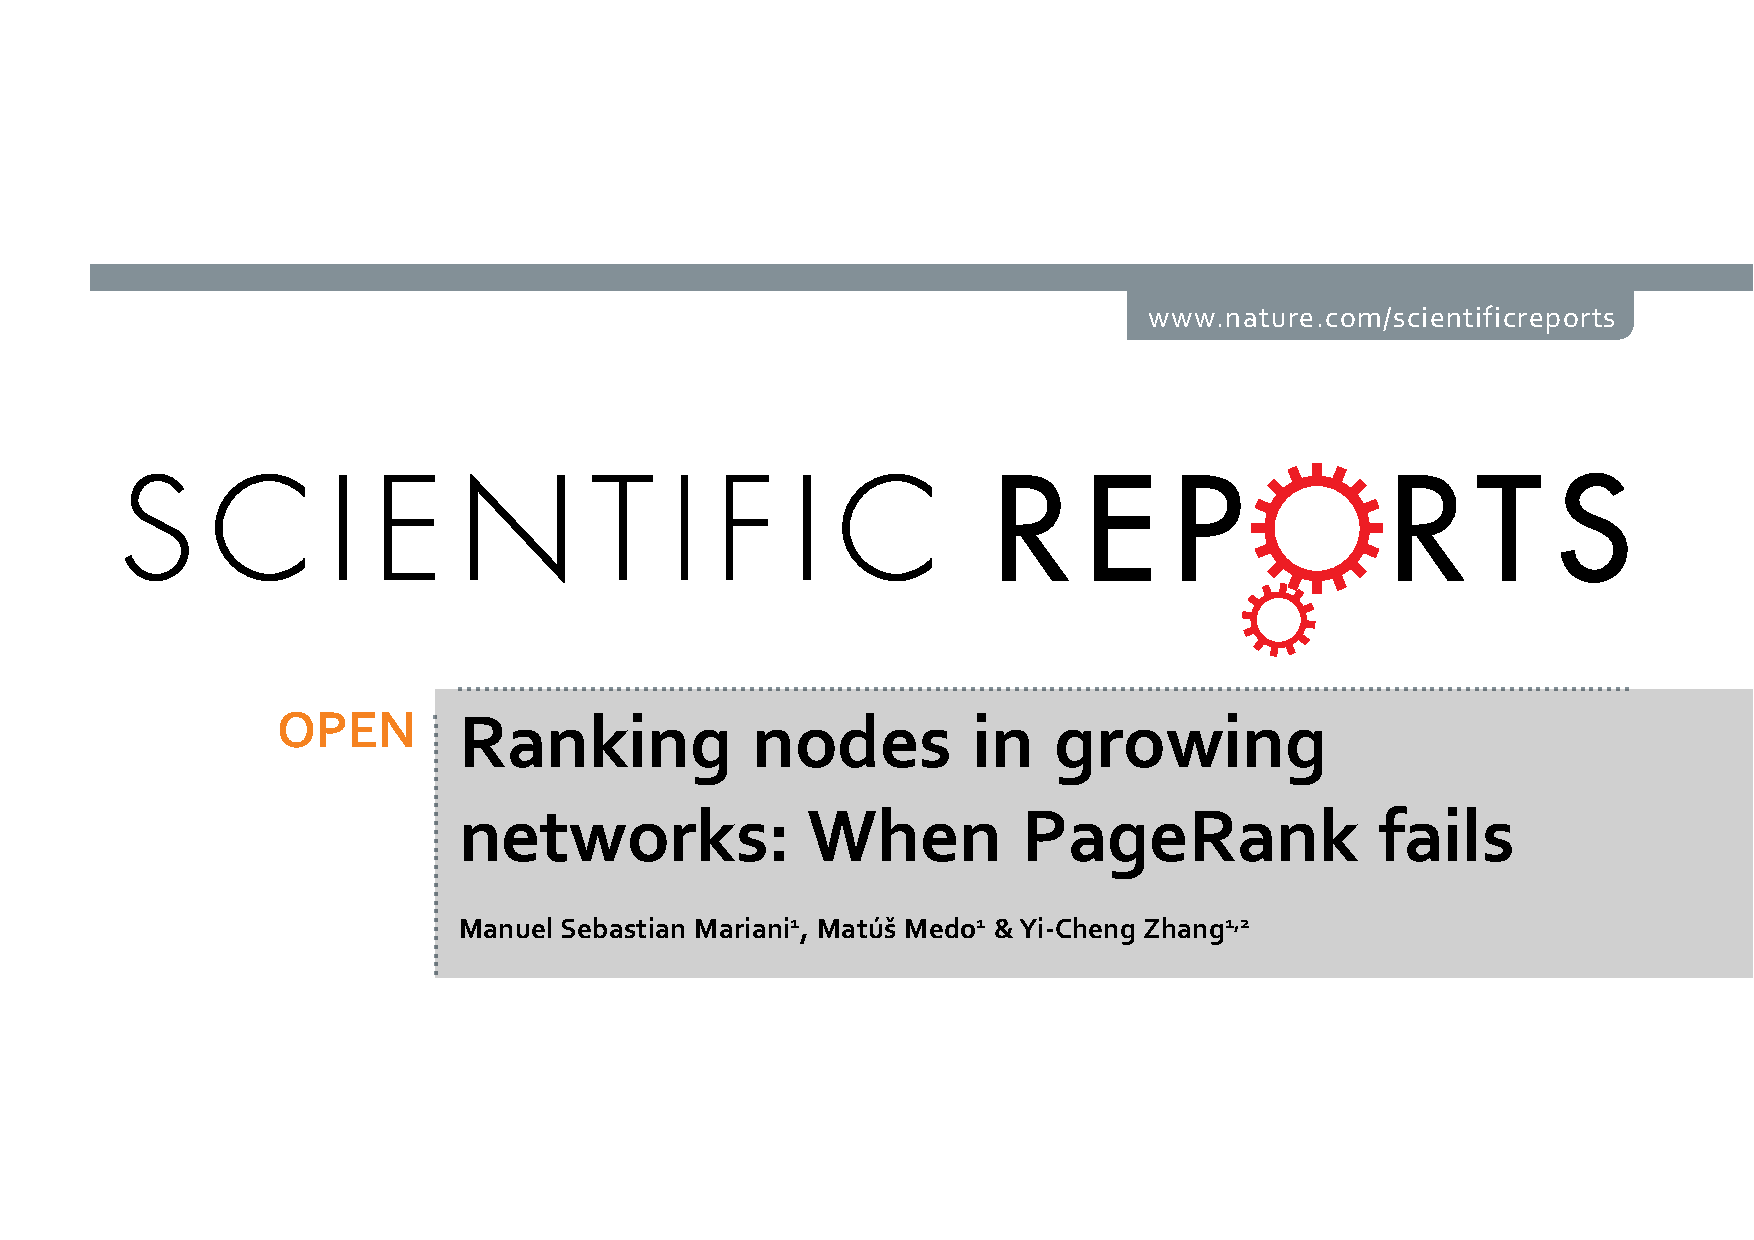
\includegraphics[width=1.0\textwidth]{figures/Header}
    \end{figure}

    Published on \emph{Nature Scientific Reports} on 10 November 2015.
\end{frame}

\begin{frame}{PageRank: recap}
    \begin{itemize}
        \item \textbf{Most popular ranking algorithm for unipartite directed networks.}
        \item Invented for Google's search algorithm
        \item Used for many other applications:
        \begin{itemize}
            \item ranking of scholarly papers
            \item ranking of images in search
            \item ranking of urban roads according to traffic flow
            \item ranking in protein interaction network
            \item etc.
        \end{itemize}
        \item \textbf{A node is important if it is pointed by other important nodes.}
    \end{itemize}
    \[
        p_{ij} = (1-\gamma) \frac{w_{ij}}{s_i^{out}} + \gamma \frac{1}{N}
    \]
\end{frame}

\begin{frame}{One PageRank fits all?}
    What is the relation between PageRank's efficacy and the properties of the network?
    \begin{itemize}
        \item PageRank: \alert{static} approach
        \begin{itemize}
            \item PageRank discards temporal information
            \item works as if nodes appear all at the same time
            \item well-known bias towards old nodes
        \end{itemize}
        \item Theoretical models and real networks can exhibit \\ \alert{strong temporal patterns}.
    \end{itemize}
    \begin{center}
        \textbf{Are there circumstances under which \\ the algorithm is doomed to fail?}
    \end{center}
\end{frame}
